%\documentclass[aps,letterpape,10pt]{revtex4}
\documentclass[aps,letterpaper,10pt]{article}
%\documentclass{article}

\usepackage{graphicx} % For images
\usepackage{float}    % For tables and other floats
%\usepackage{verbatim} % For comments and other
\usepackage{amsmath}  % For math
\usepackage{amsthm}     % For more math and proofs
\usepackage{amssymb}  % For more math
\usepackage{fullpage} % Set margins and place page numbers at bottom center
\usepackage{subfig}   % For subfigures
\usepackage[usenames,dvipsnames]{color} % For colors and names
\usepackage{fancyhdr} %headers
\usepackage{listings} %for code
\usepackage{color} %to color code
%\usepackage{wrapfig} % for inline images
\usepackage[usenames,dvipsnames,svgnames,table]{xcolor} % for more colors


%% Color and code setup
\definecolor{dkgreen}{rgb}{0,0.6,0}
\definecolor{gray}{rgb}{0.5,0.5,0.5}
\definecolor{mauve}{rgb}{0.58,0,0.82}
\definecolor{codebg}{rgb}{.95,.95,.98}

\definecolor{light-gray}{gray}{0.75}

\lstset{ %
	language=Java,
	tabsize=4, 
	numbers=left,
	numberstyle=\footnotesize,
	backgroundcolor=\color{codebg},
	breaklines=true,
	breakatwhitespace=true,
	basicstyle=\small,
	numberstyle=\tiny\color{black},
	showstringspaces=false,
	keywordstyle=\color{blue}, 
	stringstyle=\color{dkgreen},
	commentstyle=\color{gray},
	frame=single,
	title = \texttt{\lstname}
	}

%%%%%%%%%%%%

%% HEADER FORMATING%%%%%%%%%%%%%
\pagestyle{fancy}
\headheight 24pt
\setlength{\headsep}{20pt}
\lhead{PHYS 251 - Prof. Tom Witten\\Project 1}
\rhead{A. Athanassiadis\\Due 10/8/2012}
%%%%%%%%%%%%%%%%%%%%%%%%

%% Custom Definitions%%%%%%%%%%%%%%%
\newcommand{\ttt}{\texttt}
%%%%%%%%%%%%%%%%%%%%%%%%

\begin{document}
\section{Problem 1}
\begin{center}
\begin{minipage}[h]{.85\linewidth}
\begin{tabular}{|p{\linewidth}|}
\hline
By definition the golden mean $\frac{a}{b}$ satisfies $\frac{a}{b} = \frac{a+b}{a}$. Show that the golden mean has the value $\frac{1+\sqrt{5}}{2}$. Then modify the Fibonacci program to compute and write out the ratio of each term to its predecessor. (Don't forget that you want this ratio to be a double variable.)  This $g(n)$ approaches a limit for large n. Show analytically that this limit is the golden mean defined above (hint: start from the definition: $f(n) = f(n-1) + f(n-2)$.)\\
\hline
\end{tabular}
\end{minipage}

\end{center}


\vspace{2em}
The golden ratio is defined as $\phi = \frac{a}{b} = \frac{a + b}{a}$. This ratio can be solved for algebraically:
\begin{eqnarray*}
  a^2 & = & ab + b^2 \\
  a^2 - ab - b^2 & = & 0\\
  a & = & \frac{b \pm \sqrt{b^2 + 4b^2}}{2}\\
  \phi =  \frac{a}{b} & = & \frac{1 + \sqrt{5}}{2}.
\end{eqnarray*}

In the last step, the plus sign was taken in order to keep with the definition that $\phi>0$.\\

The Fibonacci sequence is given by 
\begin{displaymath}
  f(n) = \left\{
  \begin{array}{ll}
    1 &  n=0,1\\
    f(n-1) + f(n-2) & n>1
  \end{array}\right.
\end{displaymath}

Consider the ratio $$r(n) = \frac{f(n)}{f(n-1)}.$$ Assume that $\lim_{n\to\infty}r(n)=c$. Claim that $c=\phi$.\\

%% could be done formally with \epsilon-\delta
\begin{proof}
({\em Informal}) As $n$ is arbitrarily large, additionally assume $$\frac{f(n+1)}{f(n)} = \frac{f(n)}{f(n-1)} = c.$$ Then,
\begin{eqnarray*}
  c & = & \frac{f(n+1)}{f(n)}\\
    & = & \frac{f(n-1) + f(n)}{f(n)}\\
    & = & \frac{1}{c} + 1\\
  c^2 - c - 1 & = & 0\\
  c & = & \frac{1 + \sqrt{5}}{2}\\
  c & = & \phi
\end{eqnarray*}
\end{proof}

\newpage
\section{Problem 2}
\begin{center}
\begin{minipage}{.85\linewidth}
\begin{tabular}{|p{\linewidth}|}
\hline
Define a variable of type double to be the theoretical golden mean from the previous problem (to take the square root, use Math.sqrt) . Modify Fibonacci once again to display the difference between j/i and the golden mean.  Let us call this difference for the n'th Fibonacci number q(n).  We know from the previous problem that q(n) is supposed to approach zero as n gets large.  But how does it approach zero?  Plot q(n) vs n for n ranging from 3 to 20.  You don't have to use the computer to make the plot.  By plotting log q(n) vs n, test the hypothesis that q diminishes exponentially with n i. e. q(n) = (constant) exp(-n/N), where N is some ``decay constant''.  From your graph, obtain an approximate value of N if this makes sense.  You can use Java to take natural logs by using the function Math.log(number). 
You should also save the results to a file. This file should be handed in with the other files of you solution. If you have access to and are familiar with a program like Excel, MatLab, gnuPlot, etc., you can use those to plot your output for you.\\
\hline
\end{tabular}
\end{minipage}
\end{center}

For this problem, I modified the source code from Problem 1 to calculate $|\phi - r(n)|$ (modified source code included below and in folder P2). This difference should approach zero as n gets large, as indicated by the previous proof. The results of this calculation are plotted in Figure \ref{fig: convergence}. The data is provided in the table beside the plot, and is accessible in the file \ttt{P2/output.txt}. 


\begin{figure}[!h]
\begin{minipage}[!h]{.85\linewidth}
\centering
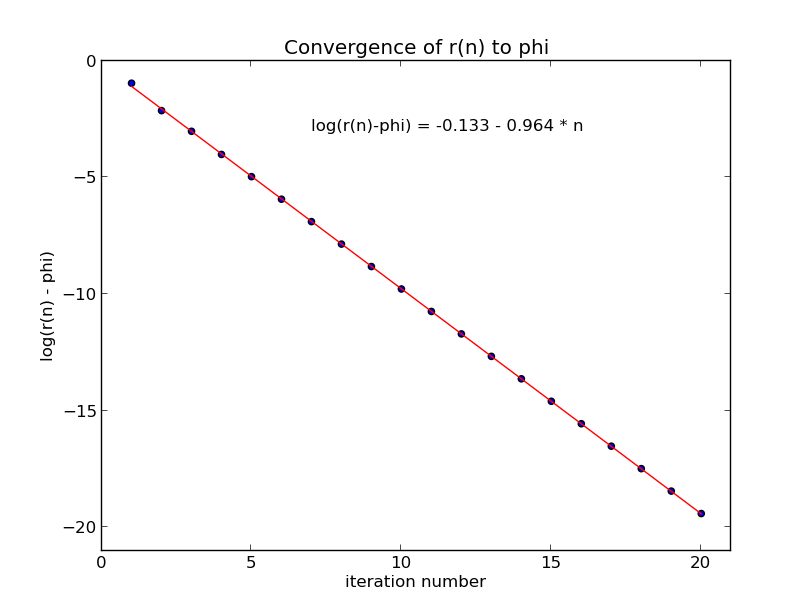
\includegraphics[width=.85\textwidth]{P2/output.png}
\caption{Convergence Plot}
\label{fig: convergence}
\end{minipage}
\begin{minipage}[!h]{.14\linewidth}
\begin{tabular}{|l|l|}
\multicolumn{1}{c}{$n$} & 
\multicolumn{1}{c}{$q = |r(n)-\phi|$} \\
\hline
1 & 3.82e-01 \\
\hline
2 & 1.18e-01 \\
\hline
3 & 4.86e-02 \\
\hline
4 & 1.80e-02 \\
\hline
5 & 6.97e-03 \\
\hline
6 & 2.65e-03 \\
\hline
7 & 1.01e-03 \\
\hline
8 & 3.87e-04 \\
\hline
9 & 1.48e-04 \\
\hline
10 & 5.65e-05 \\
\hline
11 & 2.16e-05 \\
\hline
12 & 8.24e-06 \\
\hline
13 & 3.15e-06 \\
\hline
14 & 1.20e-06 \\
\hline
15 & 4.59e-07 \\
\hline
16 & 1.75e-07 \\
\hline
17 & 6.70e-08 \\
\hline
18 & 2.56e-08 \\
\hline
19 & 9.77e-09 \\
\hline
20 & 3.73e-09 \\
\hline
\end{tabular}
\end{minipage}
\end{figure}

As expected, $r(n)$ converges to $\phi$ exponentially with a fitted decay constant of $\delta = -0.964$. Thus,$$r(n) = -.133e^{-.964n}.$$
\newpage

\section{Drawing}
Figure \ref{fig: draw} a screenshot of the drawing I made using the P251 helper class. The .java file I used to produce this is listed below Fibo.java.

\begin{figure}[!h]
\centering
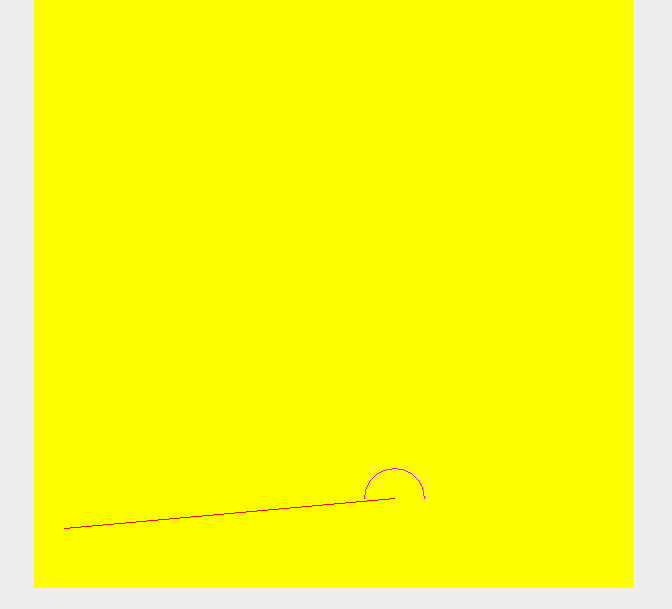
\includegraphics[width=.4\textwidth]{Draw/draw.png}
\caption{Screenshot of drawing}
\label{fig: draw}
\end{figure}

\newpage
\section{Appendix: Source Code}
\lstinputlisting{P2/Fibo.java}
\newpage
\lstinputlisting{Draw/Drawing.java}
\end{document}

%%%%%%%%%%%%%%%%%%%%%%%%%%%%%%%%%%%%%%%%%%%%%%%%%%%%%%%%
%% Reference for figures and source code
%%%%%%%%%%%%%%%%%%%%%%%%%%%%%%%%%%%%%%%%%%%%%%%%%%%%%%%%
%%
%%
%% \begin{figure}[!h]
%% \centering
%% \subfloat[Original Image]{\label{fig:5-1a}\includegraphics[width=.30\textwidth]{img_distance.png}}\hspace{20px}
%% \subfloat[Distance-Mapped Image]{\label{fig:5-1b}\includegraphics[width=.30\textwidth]{5-1a.png}} \hspace{20px}
%% \subfloat[Overlay Image]{\label{fig:5-1c}\includegraphics[width=.30\textwidth]{5-1b.png}}
%% \caption{2-Pass Distance Transform}
%% \label{fig:5-1}
%% \end{figure}

%% In this problem, I applied the two-pass distance transformation as described in class.  Figure \ref{fig:5-1a} shows the original image.  Figure \ref{fig:5-1b} shows the output of the output of the distance transform.  Figure \ref{fig:5-1c} shows an overlay of the two to confirm appropriate output.  The code used for this problem is contained in \ttt{problem1.py} and \ttt{distT.py}

%% \lstinputlisting{problem1.py}
%% \newpage
%% \lstinputlisting{distT.py}
